\documentclass[tc]{dinfunisc-propostatc}
\usepackage[T1]{fontenc}
\usepackage[utf8]{inputenc}   % pacote para acentuação
\usepackage{graphicx}
\usepackage{times}
\usepackage{colortbl}
%\usepackage[table]{xcolor}

\title{Reconhecimento ótico de caracteres implementado em arquitetura reconfigurável}

\author{}{Fabiano Kist}
\advisor[Prof. Me.]{}{Marcio Alexandre Pacheco}
\reviewer{~Prof.~Dr. Rolf Fredi Molz} {}
\reviewer{~Prof.~Dr. Rafael Ramos dos Santos }{}
%\reviewer{~Prof. ~Dr. Cara da banca 4}{}


\location{Santa Cruz do Sul}{RS}

\begin{document}

\maketitle

%deve-se usar chapter* para nao ter numero na pagina.
\chapter{resumo} Sistemas de processamento de imagens requerem um grande poder
computacional quando utilizadas em um processador de propósito geral.
Aplicações desse tipo utilizam pequenas partes do conjunto de instruções de um
processador. Este trabalho propõe a implementação de um sistema de reconhecimento
ótico de caracteres(OCR) em imagens digitais utilizando hardware
reprogramável com sistema de captura de imagens. Esta metodologia foi
desenvolvida por \cite{PACHECO} e encontra-se protegida pelos
direitos de propriedade intelectual sob o número 0000270607032603. O modelo
terá integração entre hardware e software em um sistema embarcado.  Esse
sistema pretende, além de aumentar o desempenho em relação a um sistema de OCR
tradicional, ter baixo consumo. Ambas implementaçãoes serão comparadas com o
objetivo de confrontar o desempenho e o consumo de energia com a execução dos
algoritmos em PC e FPGA XILINX Virtex-5 modelo XC5VLX110T®.




\chapter{Introdução}

	A visão e a audição são os dois principais meios pelos quais os seres
	interpretam os sinais do mundo exterior \cite{LIM}. O interesse em
	métodos de processamento de imagens digitais decorre de duas áreas
	principais de aplicação: melhoria de informação visual para a
	interpretação humana e o processamento de dados de cenas para percepção
	automática através de máquinas.

Foi no século 20 que aconteceu uma das primeiras aplicações da utilização de
técnicas de processamento de imagens e tinha como principal objetivo melhorar
as imagens digitalizadas para jornais.  Essas digitalizações posteriormente
eram enviadas por meio de cabo submarino entre Londres e Nova Iorque. O tempo
necessário para esta transmissão era de uma semana e o sistema Bartlane de
transmissão de imagens por cabo submarino (como foi chamado) conseguiu reduzir
a transmissão para três horas.

Avanços expressivos na área vieram apenas com o advento dos computadores
digitais trinta décadas mais tarde \cite{GONZALES}.  Em 1964, fotos da lua enviadas pela
missão Ranger 7, foram processadas com o objetivo de corrigir vários tipos de
distorções inerentes à câmera utilizada. Estas técnicas serviram como base para
métodos de aprimoramento de realce e restauração de imagens de outros programas
espaciais posteriores como as expedições tripuladas da série Apollo \cite{GONZALES}.

Desde a década de 60 o processamento digital de imagem vem crescendo
substancialmente. Além das aplicações no programa espacial, técnicas de
processamento de imagens são atualmente utilizadas para resolver tarefas do
cotidiano.  Embora não relacionadas com freqüência, essas tarefas comumente
requerem métodos capazes de melhorar a informação visual para a análise e
interpretação humana.  Desta forma, dentro do campo de processamento de
imagens, a integração e validação de um sistema de reconhecimento de
caracteres é uma tarefa complexa e será melhor explicado no decorrer do TC.



\chapter{Motivação}

Sistemas de processamento de imagem necessitam de grande poder computacional.
FPGA's podem oferecer esse processamento por criar \textit {hardware} dedicado
para resolver determinado tipo de tarefa. Sistemas de reconhecimento automático de
placas tornaram-se a solução em Sistemas Inteligentes de Transportes (SIT), em
que a visão artificial e padrões de reconhecimento são extensivamente aplicados
\cite{GUANGZHI}.

A identificação de veículos através do reconhecimento da placa veicular já era
usada na década de 50, tendo como objetivo o estudo do tempo de duração de
viagens entre origem e destino de veículos automotores. Os métodos iniciais
utilizavam observadores para anotar em papel, ou fitas gravadas, as placas dos
veículos e os tempos correspondentes à viagem, que depois eram comparadas
manualmente.

Desta forma, a necessidade de analisar imagens é de extrema importância para
automatizar processos. Assim, pode-se citar exemplos de aplicações de um
sistema de identificação automática de veículos no controle do tráfego; no
reconhecimento de veículos em situação irregular; no conrole de pedágios,
estacionamentos, aeroportos e intersecções; na administração de entradas
privativas; no pagamento automático de bilhetes.



\chapter{Objetivo} O objetivo deste estudo está na concepção, validação e
avaliação de um sistema completo para reconhecimento de placas de veículos.
Isso é possível através da aplicação de conceitos que envolvem a criação de
sistemas embarcados, \textit{System-on-Chip}, processamento de imagem, redes
neurais e linux.  Este trabalho será baseado na tese de mestrado de Pacheco
\cite{PACHECO}, que desenvolveu uma nova metodologia de localização de
regiões
 candidatas em imagens digitais utilizando arquiteturas
reconfiguráveis. A meta
 é utilizar o modelo já implementado em VHDL para
criar um sistema completo de OCR.  Este trabalho de conclusão de curso tem como
finalidade fazer a integração e
 validação de um sistema que faça a captura de
imagem, extraia as regiões candidatas da placa contidas em
 uma imagem
digital, extrair os caracteres e faça o reconhecimento através da
 aplicação
de redes neurais.

A metodologia empregada para executar a tarefa de captura de imagem,
localização da placa, extração dos caracteres e reconhecimento 
faz uso
 de diferentes técnicas de processamento e análise de
imagens. Desta forma, o
 objetivo final deste trabalho é validar
primeiramente o OCR em software e
 posteriormente em \textit{hardware}.
 Todas as etapas
do modelo proposto serão validadas em \textit{Field Programmable Gate Array}
(FPGA) visando obter
 melhores desempenhos de processamento da imagem.  As
tarefas que executam as
 funções de extração de bordas, marcação dos pontos e
filtragem dos mesmos, serão executadas dedicadamente, sendo essa, uma das
principais características da arquitetura utilizada. 
 

\chapter{Metodologia} \section*{Elementos do processamento e análise de imagem}
Os principais dispositivos de exibição usados nos modernos sistemas de
processamento de imagens são os monitores de televisão (TV), monocromáticos e
coloridos.  Além desses, incluem-se na lista dos equipamentos responsáveis pela
apresentação dos resultados das aquisições de imagens, os tubos de raios
catódicos e dispositivos de impressão \cite{LIM}. A Figura \ref{fig:elemProc}
apresenta o modelo proposto para um sistema de processamento e análise de
imagem.



\begin{figure}[ht] \centering 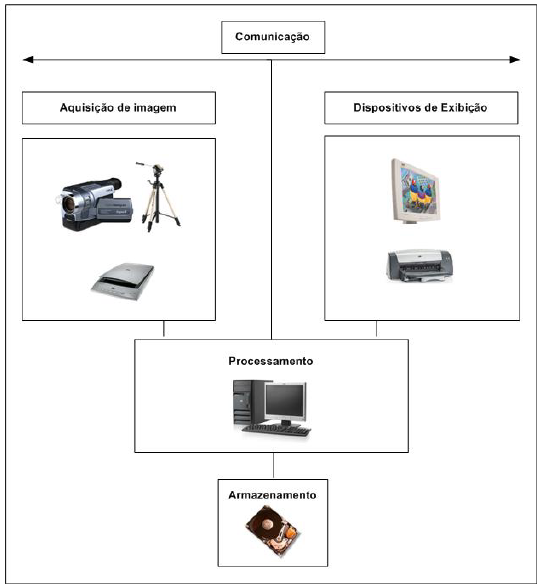
\includegraphics[scale=0.7]{figures/elemProc.png}
	\caption{Elementos do processamento e análise de imagem. Fonte: \cite{PACHECO} }
	\label{fig:elemProc} \end{figure}


\section*{Placa de prototipação alvo} A prototipação do sistema será realizada
utilizando com alvo a placa  XUPV5-LX110T, que posui o FPGA  XC5VLX110T da
família \textit{Virtex-5}. Além do FPGA a placa oferece diversos outros
recursos para aplicaçãoes avançadas, como rede giga-bit, porta sata,
\textit{usb-host}, processador \textit{ Open-Sparc}, dentre outros
\cite{XILINX}.  A placa também oferece estruturas de memória que serão
extremamente importantes para a concepção, visto que tanto o sistema
operacional e os módulos descritos em HDL farão uso da mesma.  
A Figura \ref{fig:placa} mostra os recursos que se pretende utilizar no estudo. Além dos 
recursos fornecidos pela placa também será necessário uma placa de captura usb e uma câmera.

\begin{figure}[ht] \centering 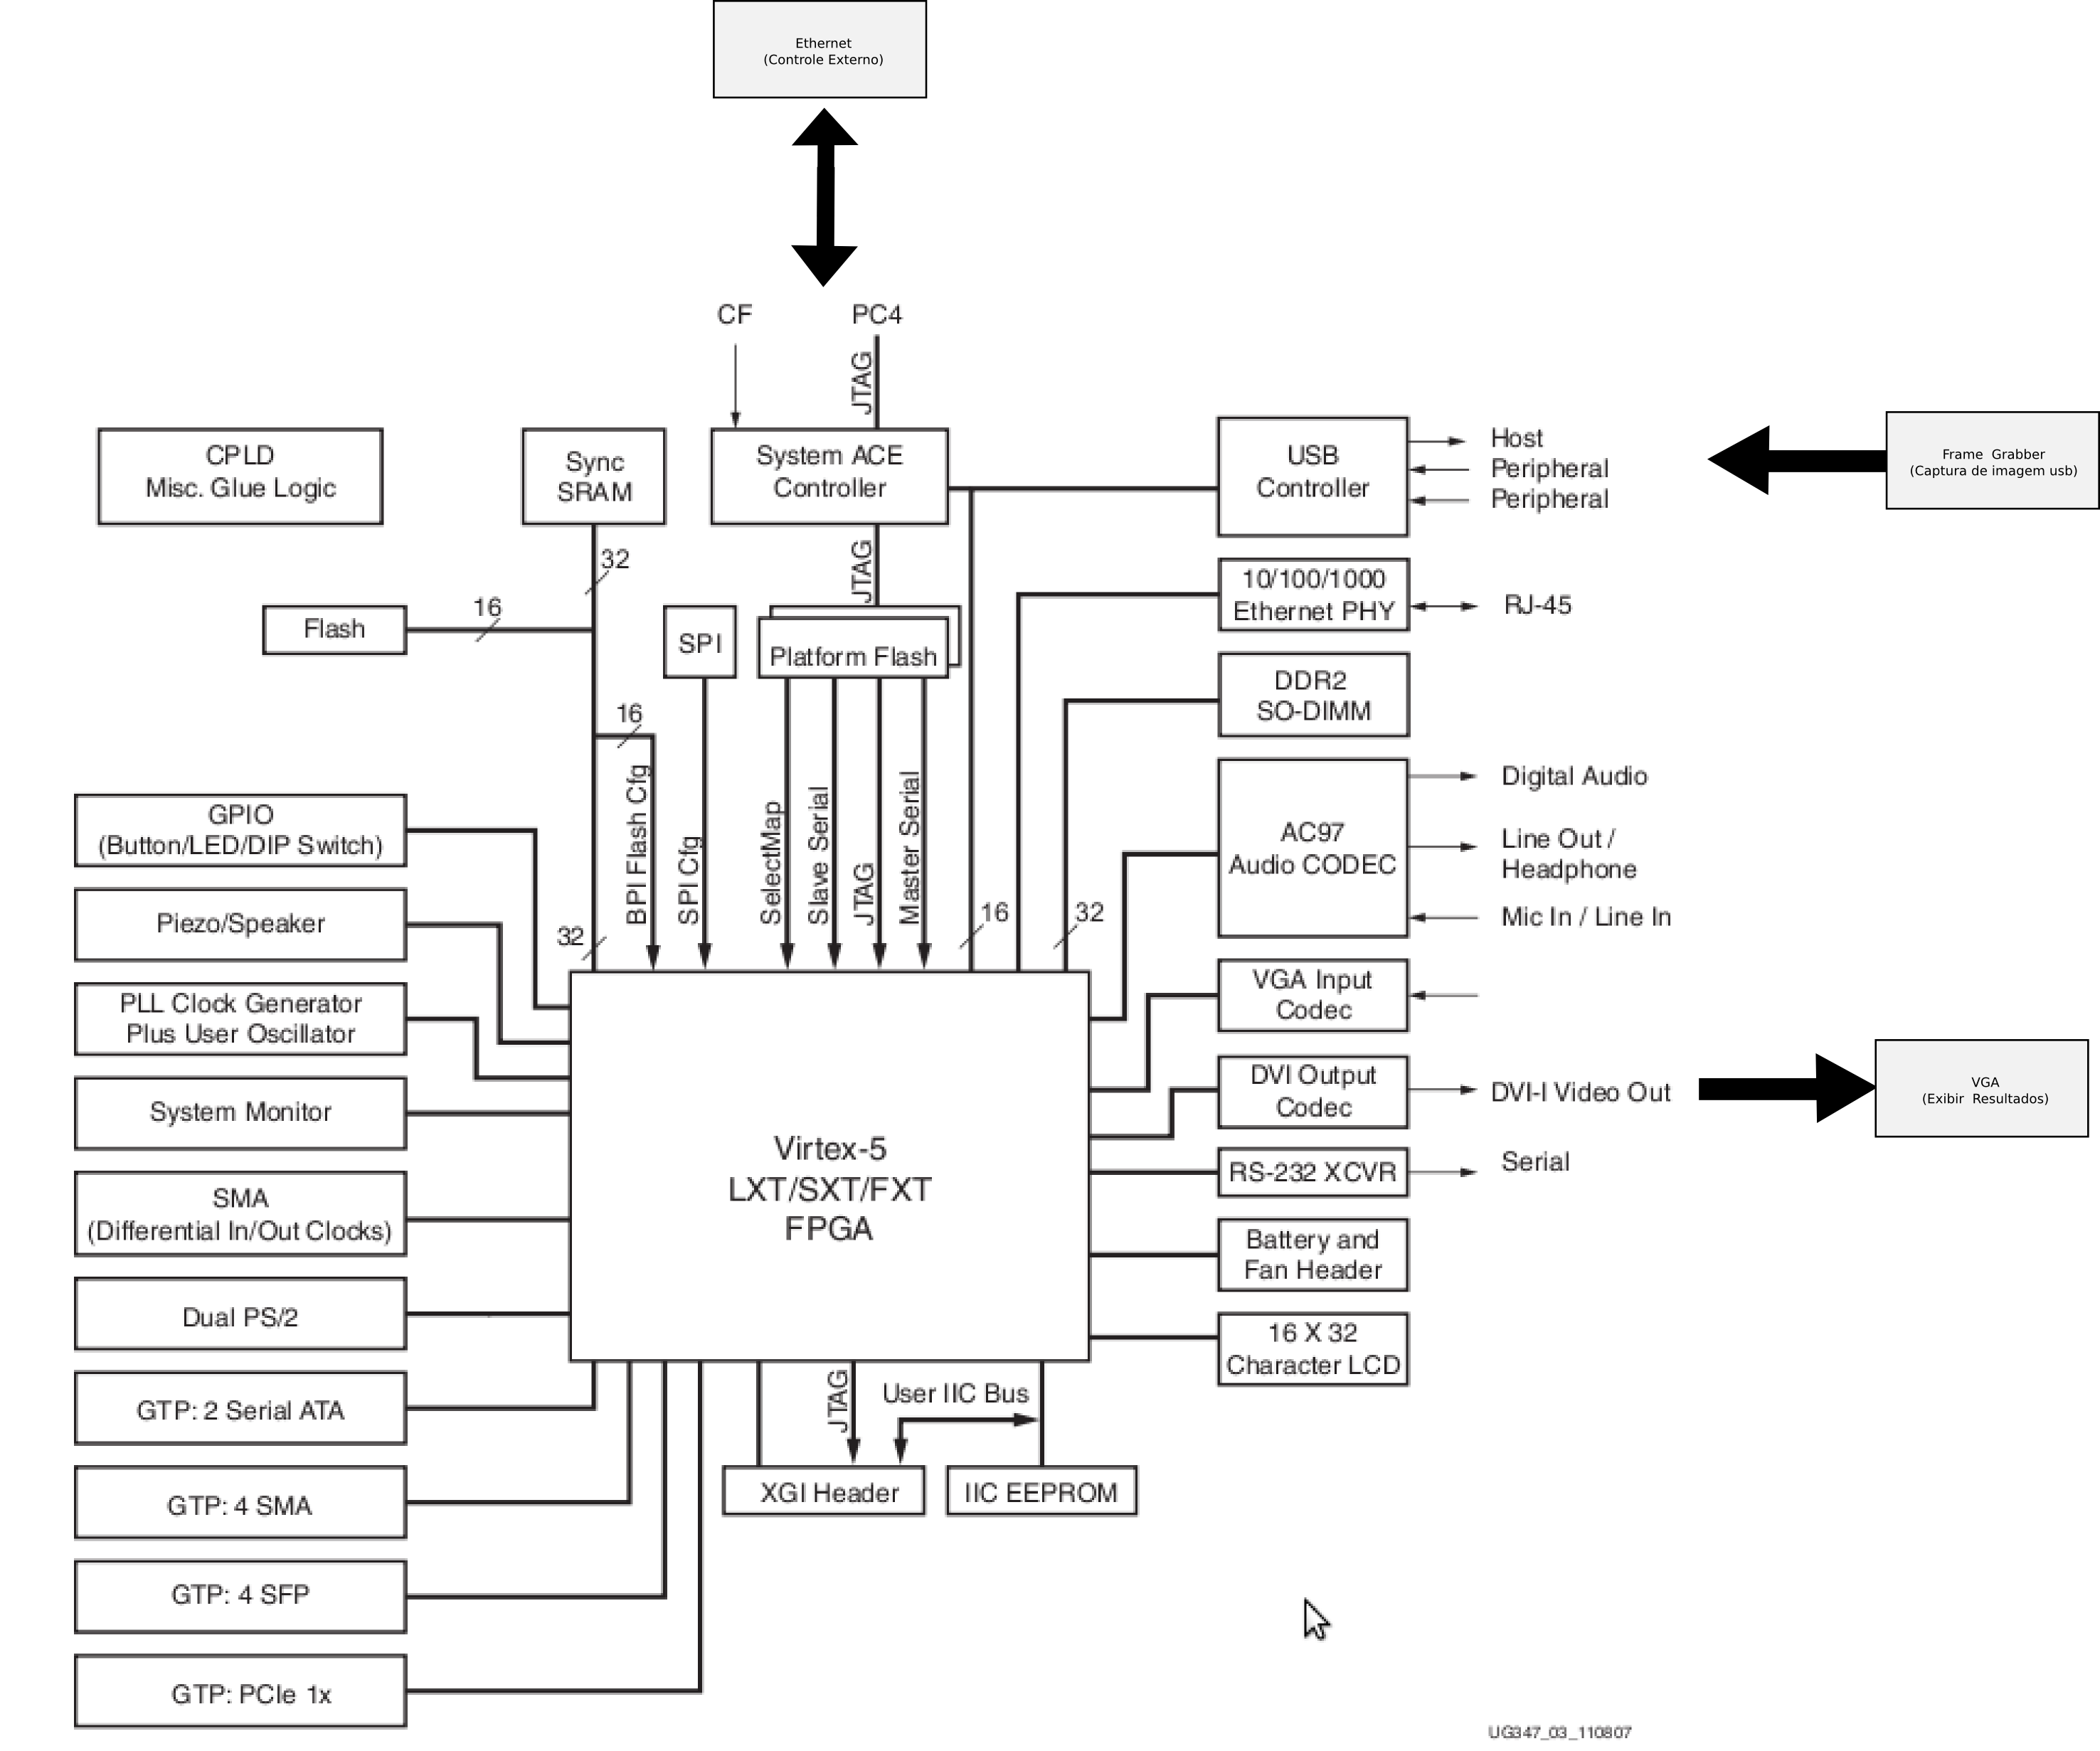
\includegraphics[scale=0.8]{figures/recursos.png}
	\caption{Plataforma de desenvolvimento Virtex-V , da \textit{Xilinx}.
	Fonte: \cite{XILINX}} \label{fig:placa} \end{figure}

\section*{Modelo Proposto} O objetivo deste estudo é criar um sistema
com base na implementação desenvolvida por Márcio Alexandre Pacheco, integrando a
etapa de captura de imagem e reconhecimento por redes neurais. 

\begin{figure}[ht] \centering 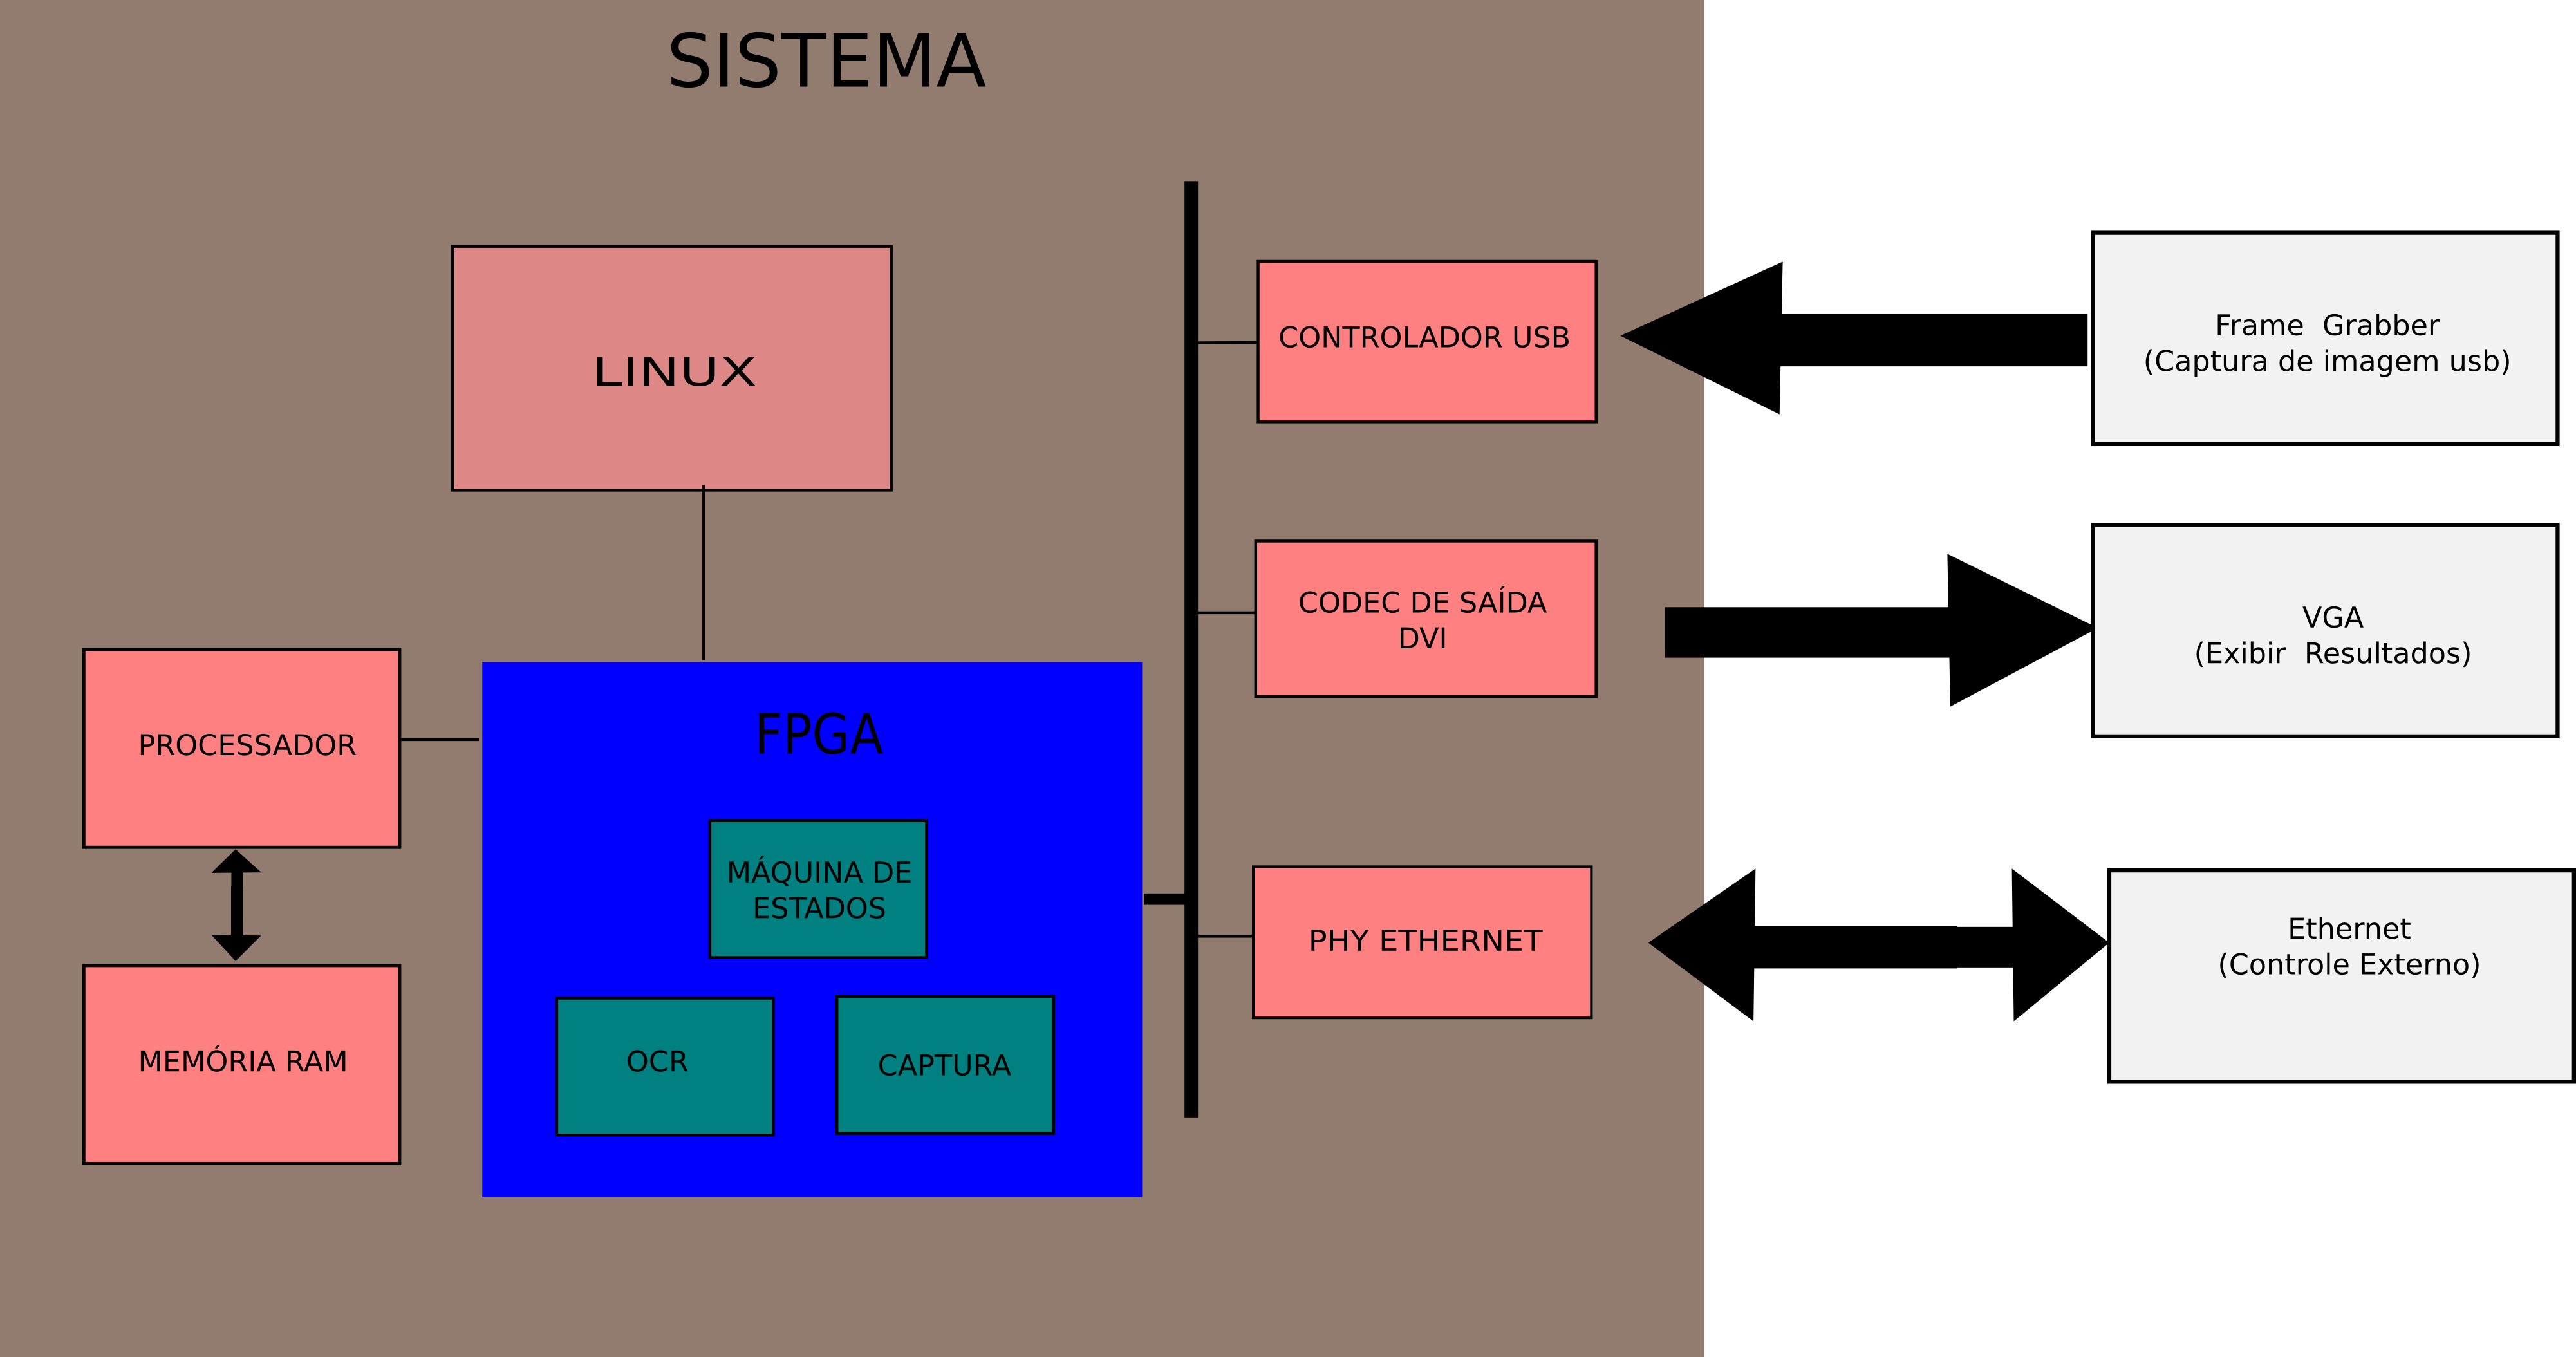
\includegraphics[scale=0.6]{figures/sis.png}
	\caption{Sistema Proposto} \label{fig:sisProp} \end{figure}

Dentro do FPGA estará a máquina de estados que fará o controle de toda a
análise de imagem, sendo iniciada através de um estimulo externo gerado por um
pino de IO. A imagem que será analisada será capturada por uma câmera acoplada
a um \textit{frame-grabber}, que é um dispositivo para captura de imagens pela
porta \textit{usb}.

A imagem será enviada através do barramento para o FPGA, que armazenará os
dados na memória. O FPGA consome os dados do modelo para obter o total de regiões
candidatas, extração e reconhecimento dos caracteres.  A
Figura \ref{fig:sisProp} mostra a arquitetura do dispositivo.

	\section*{Estratégia de validação do sistema a ser implementado} A
	validação do sistema será realizada com o método típico para validação
	de módulos em \textit{hardware} sendo comparado o desempenho em suas respectivas arquiteturas. 
  Após a integração de todos os módulos os resultados serão comparados ao OCR já implementado em PC e que 
  faz uso dos mesmos algoritmos de extração de regiões candidatas, extração de caracteres e reconhecimento através de redes neurais.
	

\chapter{Cronograma}

O desenvolvimento deste trabalho se dará da seguinte forma:

\begin{enumerate}
	\item \label{ela-pro} Elaboração da proposta de TC.
	\item \label{anI} Análise dos métodos de localização de regiões candidatas em imagens digitais e
		reconhecimento de caracteres através de redes neurais.
	\item \label{anII} Análise do funcionamento de OCR's já homologados em PC.
	\item \label{anIII} Análise dos modelos implementados em hardware estudados no item III. 
	\item \label{dI} Estudo do Linux Embarcado.
	\item \label{dII}  Validação dos módulos de localização de regiões candidatas.
	\item \label{dIII} Implementação do módulo de caputra de imagem. 
	\item \label{esc-tcI}  Escrita do TC I.
	\item \label{imI} Implementação da máquina de estados para controle da análise de imagem.
	\item \label{imII} Desenvolvimento da camada de integração.
	\item \label{imIII} Integração dos módulos que compõe o sistema.
	\item \label{tec} Teste e correções.
		\subitem Comparar desempenho entre hardware e software.
	\item \label{esc-tcII} Escrita do TC II.
\end{enumerate}

\definecolor{midgray}{gray}{.5}
\begin{table}[!htbp]
	\centering
		\begin{tabular}{|c|c|c|c|c|c|c|c|c|c|c|}
		\hline
		&\multicolumn{5}{c|}{2010}&\multicolumn{5}{c|}{2010}\\
		\hline
		&MAR&ABR&MAI&JUN&JUL&AGO&SET&OUT&NOV&DEZ\\
		\hline
		\ref{ela-pro}&\cellcolor{midgray}&&&&&&&&&\\
		\hline
		\ref{anI}&&\cellcolor{midgray}&&&&&&&&\\
		\hline	
		\ref{anII}&&\cellcolor{midgray}&&&&&&&&\\
		\hline			
		\ref{anIII}&&\cellcolor{midgray}&\cellcolor{midgray}&&&&&&&\\
		\hline	
		\ref{dI}&&&\cellcolor{midgray}&&&&&&&\\
		\hline
		\ref{dII}&&&\cellcolor{midgray}&\cellcolor{midgray}&&&&&&\\
		\hline	
		\ref{dIII}&&&&\cellcolor{midgray}&\cellcolor{midgray}&&&&&\\
		\hline	
		\ref{esc-tcI}&&&\cellcolor{midgray}&\cellcolor{midgray}&\cellcolor{midgray}&&&&&\\
		\hline	
		\ref{imI}&&&&&\cellcolor{midgray}&&&&&\\
		\hline	
		\ref{imII}&&&&&&\cellcolor{midgray}&&&&\\
		\hline	
		\ref{imIII}&&&&&&\cellcolor{midgray}&\cellcolor{midgray}&\cellcolor{midgray}&&\\
		\hline	
		\ref{tec}&&&&&&&&\cellcolor{midgray}&\cellcolor{midgray}&\\
		\hline	
		\ref{esc-tcII}&&&&&&&&\cellcolor{midgray}&\cellcolor{midgray}&\cellcolor{midgray}\\
		\hline	
		\end{tabular}
\end{table}


%gambiarra para adicionar referências que não são utilizadas.
%\chapter{gambi}

\cite{Tanen}
\cite{RFC2544}
\cite{throughput}
\cite{Helvey}
\cite{networkTrafficTraces}



\bibliography{biblio}
\bibliographystyle{abnt}

\chapter{}
\makesignature
\end{document}
